\subsection{乳腺细胞的模拟}
\begin{frame}{乳腺细胞吸入实验及DPD模型}
\begin{columns}
\begin{column}[c]{0.25\textwidth}
\begin{center}
\usetikzlibrary{%
    decorations.pathreplacing,%
    decorations.pathmorphing,arrows
}
\begin{tikzpicture}
\begin{axis}[axis equal,colormap={bw}{gray(0cm)=(0); gray(1cm)=(1)}, view={0}{90},xmin=-10.25,xmax=10.25,ymin=-10.25,ymax=10.25,width=1.3\textwidth,height=1.3\textwidth,xtick=\empty,ytick=\empty,hide axis]
\addplot3 + [only marks,mark=ball,ball color=gray,draw=none,mark size=1.5pt] table[x=x,y=y,z=z]{./figures/data/sphere.vertex};
\addplot3[patch] file{./figures/data/sphere.dat};
\end{axis}
\end{tikzpicture}

\end{center}
\end{column}
\begin{column}[c]{0.75\textwidth}
{\small
\[
V(\{\mathbf{X}_i\}) = V_{\text{in-plane}} + V_{\text{bending}} + \textcolor{red}{V_{\text{area}}} + V_{\text{volume}}
\]}
\end{column}
\end{columns}
\begin{center}
\asyinclude[width=\textwidth, viewportwidth=\textwidth,viewportheight=0.3571\textwidth]{./figures/3dchannel.asy}
\end{center}
\end{frame}

\begin{frame}{乳腺细胞吸入实验的模拟动画}
\begin{center}
\begin{overpic}[width=\textwidth]{./animate/cell2d/wall.pdf}
\put(0,0){\animategraphics[width=\textwidth, poster=first,controls,buttonsize=0.8em]{5}{./animate/cell2d/}{0}{90}}
\end{overpic}
\end{center}
\end{frame}

\begin{frame}{乳腺细胞吸入实验的模拟结果}
\begin{columns}
\begin{column}[c]{0.5\textwidth}
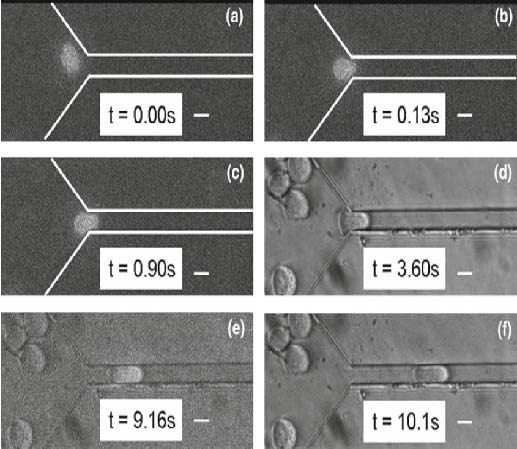
\includegraphics[width=\textwidth]{./figures/cell.jpg}
\end{column}
\begin{column}[c]{0.5\textwidth}
\begin{center}
\usetikzlibrary{%
    decorations.pathreplacing,%
    decorations.pathmorphing,arrows
}
\begin{tikzpicture}[scale=0.925]
\begin{scope}[yshift=95pt]
  \begin{axis}[xmin=-60, xmax=60, ymin=-22, ymax=22,width=182pt,height=95pt,
              ytick={-20,0,20},
              %xlabel={$t$}, 
              ylabel={$z$},
              xticklabel=\empty,
label style={anchor=near ticklabel},
    ylabel style={yshift=-2em},
    xlabel style={yshift=0.3em},
    tick label style={font=\scriptsize},
    label style={font=\footnotesize},
    legend style={font=\tiny,legend cell align=left,legend pos=north west}
              ]

   \addplot[color=black,no marks,thick] coordinates {(-70,-20.25) (-40,-20.25) (-23, -3.25) (23, -3.25) (40,-20.25) (70,-20.25)};
   \addplot[color=black,no marks,thick] coordinates {(-70,20.25) (-40,20.25) (-23, 3.25) (23, 3.25) (40,20.25) (70,20.25)};

   \addplot[no marks,ball color=red]  table[x=x1,y=y1]{./figures/data/cellshape.dat};
   \addplot[no marks, blue!25!red,thick]  table[x=x2,y=y2]{./figures/data/cellshape.dat};
   \addplot[no marks, blue!50!red,thick]  table[x=x3,y=y3]{./figures/data/cellshape.dat};
   \addplot[no marks, blue!75!red,thick]  table[x=x4,y=y4]{./figures/data/cellshape.dat};
   \addplot[no marks, blue!100!red,thick]  table[x=x5,y=y5]{./figures/data/cellshape.dat};
   \addplot[no marks, blue!75!green,thick]  table[x=x6,y=y6]{./figures/data/cellshape.dat};
   \addplot[no marks, blue!50!green,thick]  table[x=x7,y=y7]{./figures/data/cellshape.dat};
   \addplot[no marks, blue!25!green,thick]  table[x=x8,y=y8]{./figures/data/cellshape.dat};
   \addplot[no marks, green,thick]  table[x=x9,y=y9]{./figures/data/cellshape.dat};
   \addplot[no marks, red!25!green,thick]  table[x=x10,y=y10]{./figures/data/cellshape.dat};
   \addplot[no marks, red!50!green,thick]  table[x=x11,y=y11]{./figures/data/cellshape.dat};
   \addplot[no marks, red!75!green,thick]  table[x=x12,y=y12]{./figures/data/cellshape.dat};
  \end{axis}
\end{scope}

  \begin{axis}[xmin=-60, xmax=60, ymin=0, ymax=18, width=182pt,height=135pt,
              %ytick={0,30,60,90,120,150,180},
              xlabel={$x$}, ylabel={$t$},
label style={anchor=near ticklabel},
    ylabel style={yshift=-2em},
    xlabel style={yshift=0.3em},
    tick label style={font=\scriptsize},
    label style={font=\footnotesize},
    legend style={font=\tiny,legend cell align=left,legend pos=north west}
              ]
   \addplot[no marks, black,thick]  table[x=x,y=t]{./figures/data/cellx.dat};

  \end{axis}
\end{tikzpicture}

\vspace{-2em}
\end{center}
\end{column}
\end{columns}
\end{frame}


